\documentclass[a4j]{jarticle}
\title{計算科学レポート2}
\author{35-196004 天野智仁}
\date{}
\usepackage[dvipdfmx]{graphicx}	% required for `\includegraphics' (yatex added)
\usepackage{listings}
\begin{document}
\maketitle





\section{wannier90を使ったバンドのプロット}
wannier90を使って,wannier基底を使った強束縛近似によるバンド計算を実行しよう.


  \subsection{QEによる計算}
  まずはじめにscf計算を実行した.主なパラメーターはwannier90のチュートリアルから変更せず,図の値を使用した.

  \begin{lstlisting}
  smearing='cold'
  degauss=0.02
  pseudo potensial Cu.pz-n-van_ak.UPF
  K_POINTS(automatic)
   16 16 16 0 0 0
  \end{lstlisting}
  scf計算の結果得られたTotalEnergyは$-121.12133546 \mathrm{Ry}$ ,FermiEnergyは$12.2101\mathrm{eV}$であった.これを元に(001)面での電荷密度を図示したのが図\ref{170115_31May19}である.図\ref{170115_31May19}は,Cuのサイトに電子が強く局在している様子を表している.これはCuが3d金属であることに由来し,局在するd軌道の様子が表れていると考えられる.
	 \begin{figure}[htb]
	   \begin{center}
	    \begin{tabular}[tb]{c}
	\begin{minipage}[cbt]{0.5\hsize}
\begin{center}
     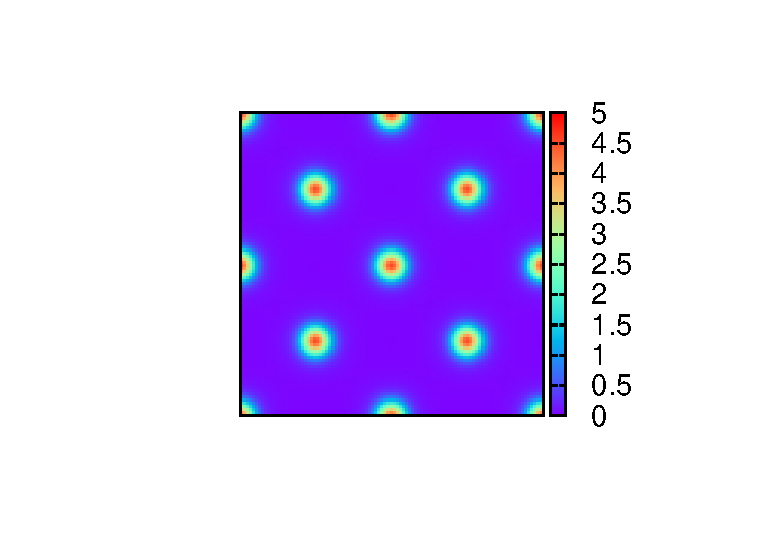
\includegraphics[width=8cm]{charge2D.eps}
     \caption{Cuの電子密度分布}
 \label{170115_31May19}
 \end{center}
	\end{minipage}
       \begin{minipage}[cbt]{0.5\hsize}
\begin{center}
      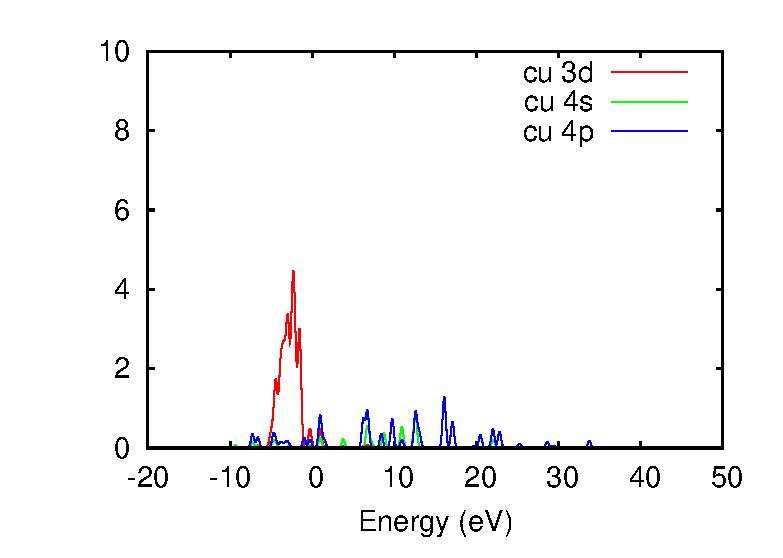
\includegraphics[width=10cm]{copper_pdos.eps}
      \caption{Cuの各軌道のDOS}
 \label{171553_31May19}
 \end{center}
       \end{minipage}
	     	    \end{tabular}
	   \end{center}
	 \end{figure}

	 このことを確かめるために,各軌道の状態密度を図\ref{171553_31May19}に示した.これを見ればわかるように,3d軌道がFermi準位の直下に強いDOSを持っており,ここに電子が沢山いることを示している.
  このことは,QEによるバンド図\ref{191823_31May19}からも確認することができる.ここではエネルギーがフェルミエネルギーを基準にして示されているが,その下$-2\mathrm{eV}$の所に集中的にあるバンドが3d軌道である.

    \begin{figure}[htb]
       \begin{center}
	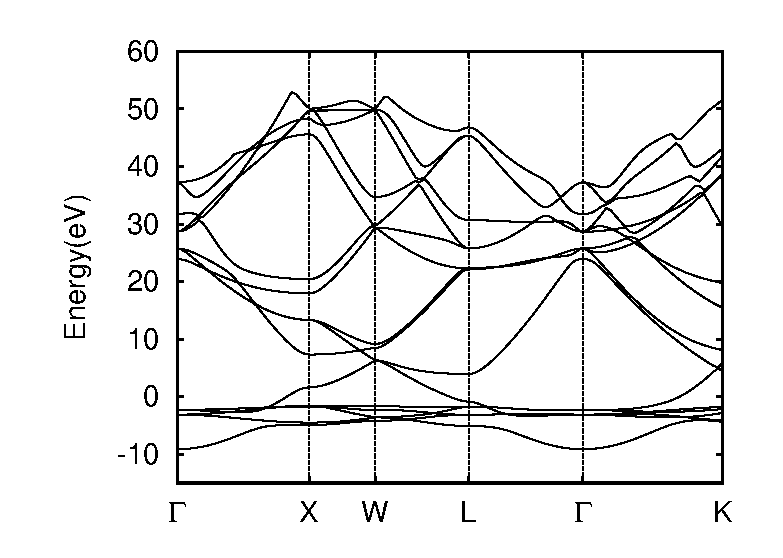
\includegraphics[width=10cm]{Cu.bands.eps}
	\caption{QEによるCuのバンド図}
	\label{191823_31May19}
       \end{center}
    \end{figure}


  以上の考察から,Cuでは,d軌道を用いた強束縛近似がバンドをQEでの計算をうまく再現することが予想される.



\subsection{wannier90の計算}
wannier90の細かい設定を記述していこう.基本的にwannier90のチュートリアルと全く同じである.
まず,バンドの数(nscfと一致)及びワニエ関数の数の指定は
\begin{lstlisting}
 num_bands = 12
 num_wann  = 7
\end{lstlisting}
とした.Outer window,Inner Windowの指定はQEのバンド図と見比べて
 \begin{lstlisting}
  dis_win_max     = 38.0
  dis_froz_max    = 13.0
  dis_num_iter    =  50
  dis_mix_ratio   = 1.0
 \end{lstlisting} 
 とした.計算ではまず,Cuのフェルミ面の計算を行った.(図\ref{192331_31May19})

   \begin{figure}[htb]
     \begin{center}
   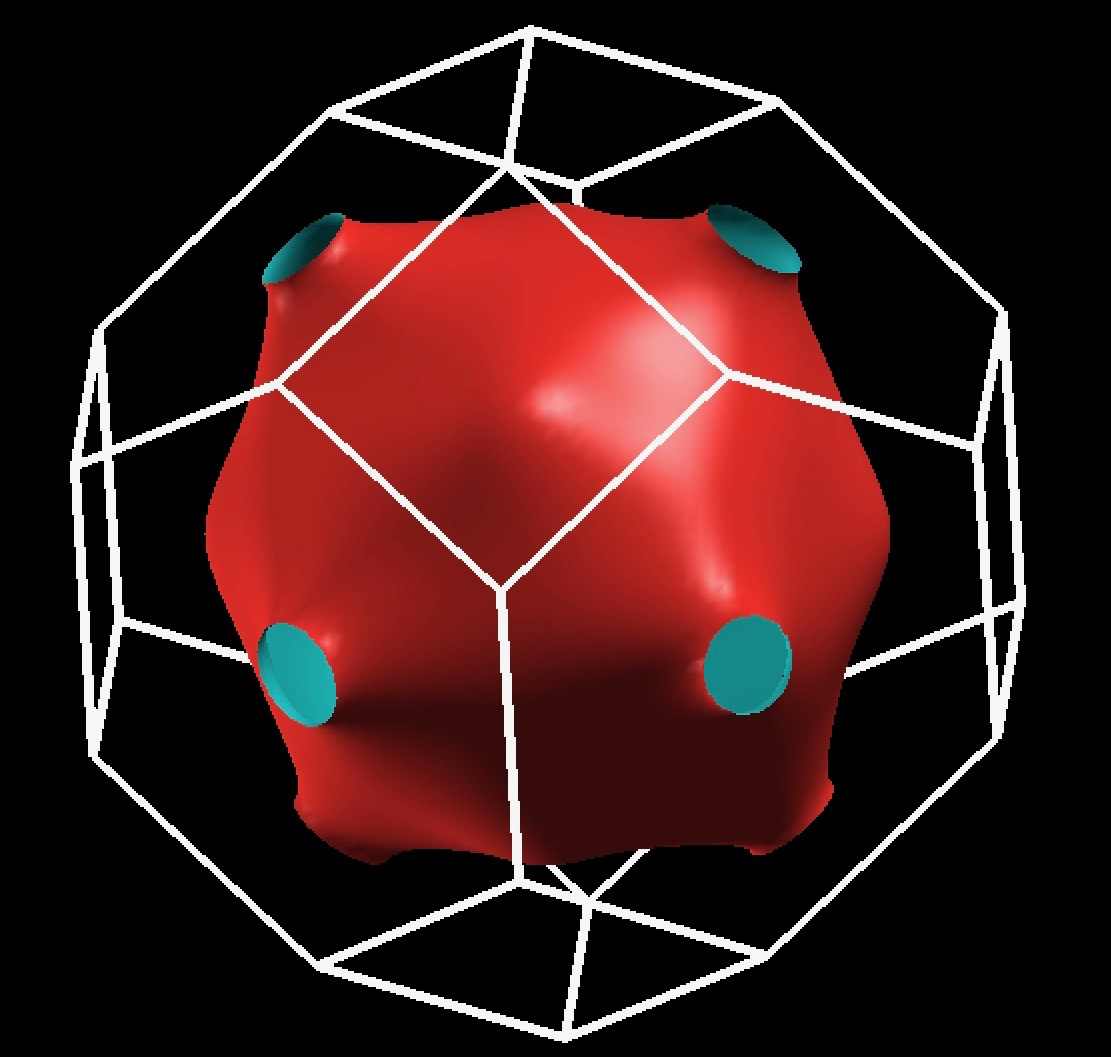
\includegraphics[bb=0 0 1111 1057,width=10cm]{fermisurface.jpg}
   \caption{Cuのフェルミ面}
      \label{192331_31May19}
       \end{center}
   \end{figure}


 

 計算の結果得られたwannierのバンド図とQEのバンド図\ref{191823_31May19}を重ねて表示したものが図\ref{195341_31May19}である.ここでは緑がQEによって得られたバンド,赤がWannier90によって得られたバンドである.
\begin{figure}[htb]
 \begin{center}
  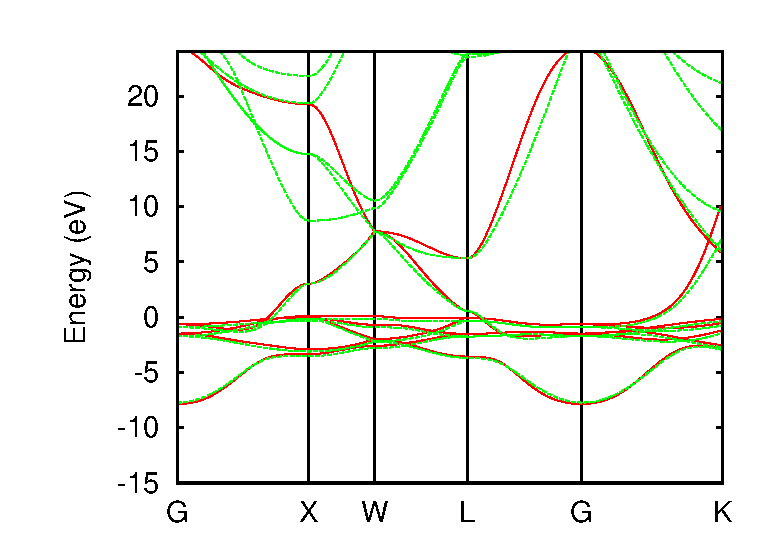
\includegraphics[width=10cm]{bandQEW.eps}
  \caption{QEとWannier90のバンド図の比較}
  \label{195341_31May19}
 \end{center}
\end{figure}







\end{document}